\chapter{Iron Activity: Irradiated to 100DPA}
\label{chap:appendixironactivity}

\section{Activity vs Beam Energy}

The beam energy was set to 5MeV, 10MeV, 15MeV, 20MeV, 25MeV and 30MeV within SRIM, and the Activity V2 code was used to calculate how radioactive each sample would be if irradiated to 100 \acrshort{dpa} of damage.

The beam settings are:

\begin{itemize}
\item target material = pure iron
\item target thickness = 0.5mm
\item beam current = 60 micro amps (maximum proton current for the Scanditronix MC-40)
\item beam area = $64mm^2$
\end{itemize}



\begin{figure}[!htb]
\centering
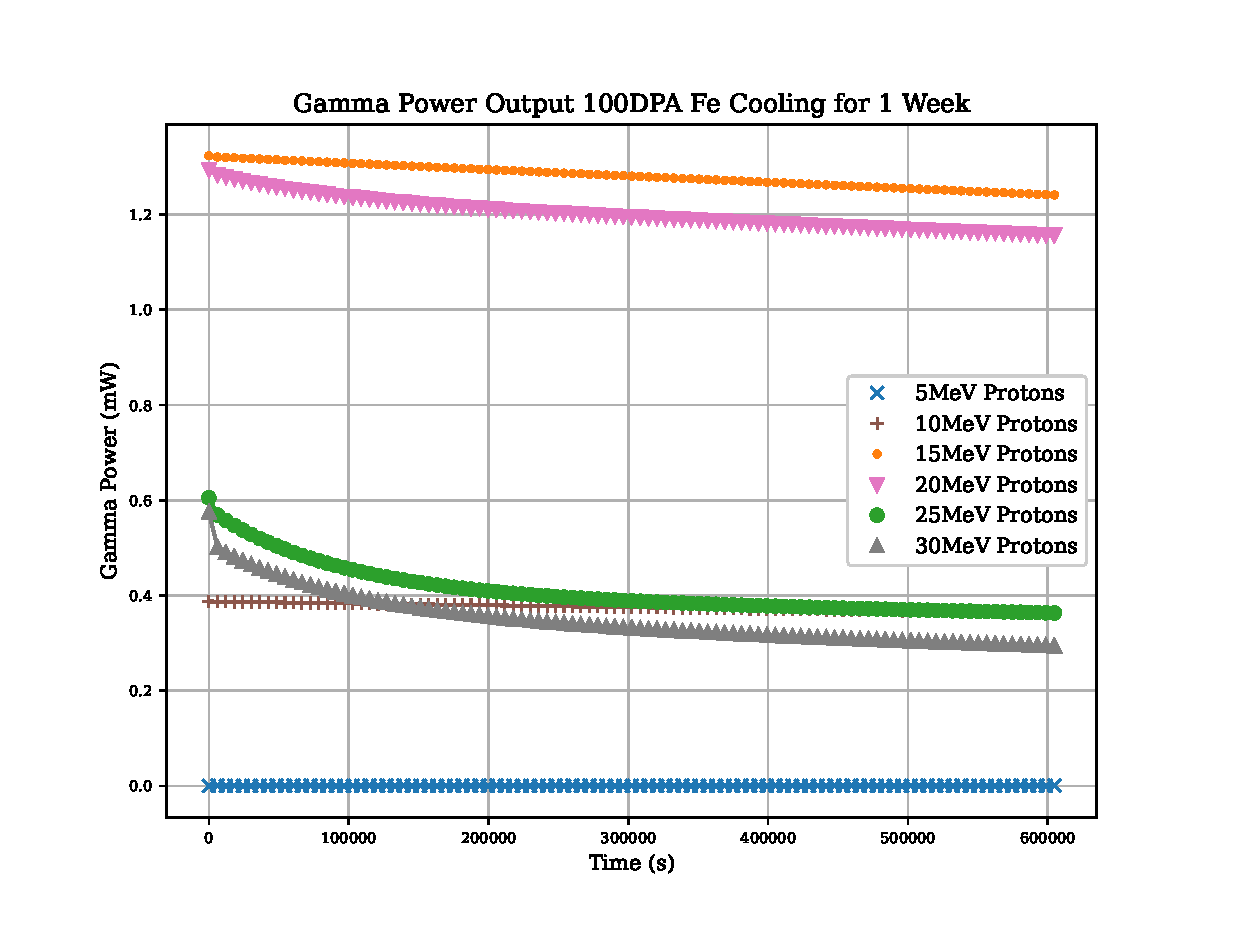
\includegraphics[width=0.7\linewidth]{chapters/activity_code/fe_100dpa/cooling.eps}
\caption{}
\label{fig:100dpa-cooling}
\end{figure}



\clearpage
\FloatBarrier
\subsection{5MeV Proton Beam - 60 microamp 100DPA}

With a proton energy of 5MeV the target must be irradiated for 205 days to reach 100DPA.

\begin{figure}[!htb]
\centering
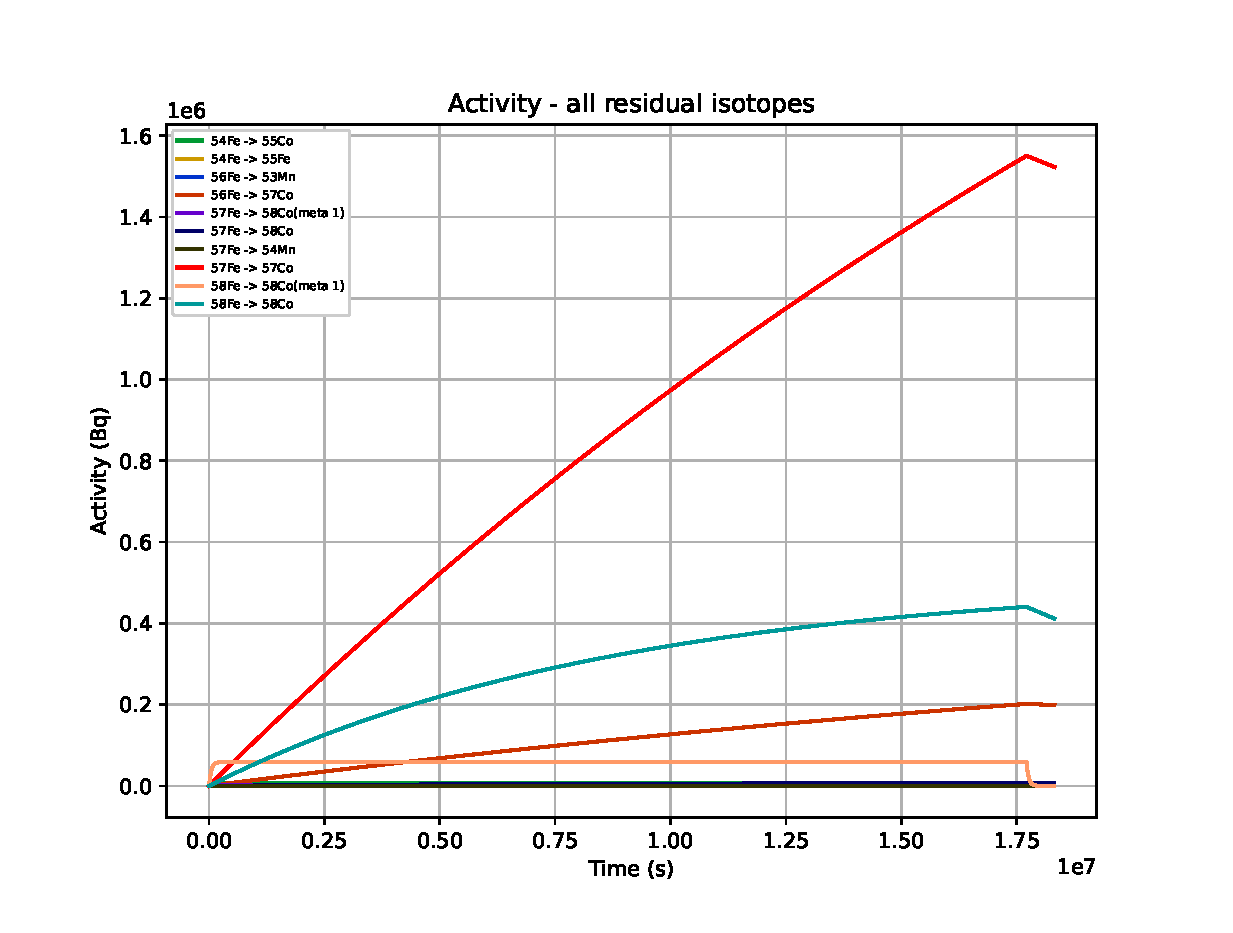
\includegraphics[width=0.7\linewidth]{chapters/activity_code/fe_100dpa/by_isotope/05MeV_all_radioactive_isotopes.eps}
\caption{}
\label{fig:5mev-proton-100dpa-activity}
\end{figure}

\begin{figure}[!htb]
\centering
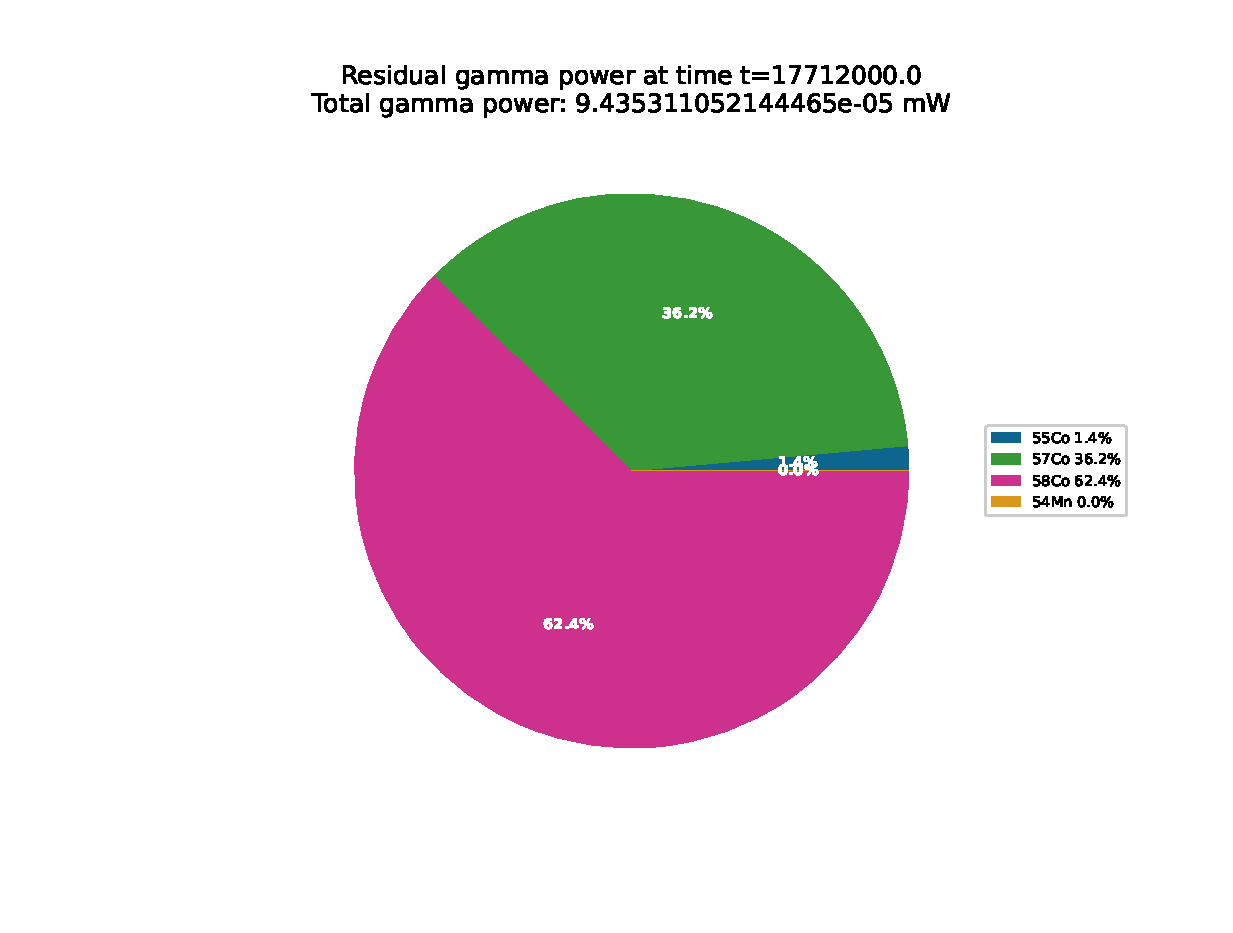
\includegraphics[width=0.7\linewidth]{chapters/activity_code/fe_100dpa/endofbeam/05MeV_0400_17712000.eps}
\caption{}
\label{fig:5mev-proton-100dpa}
\end{figure}

\begin{figure}[!htb]
\centering
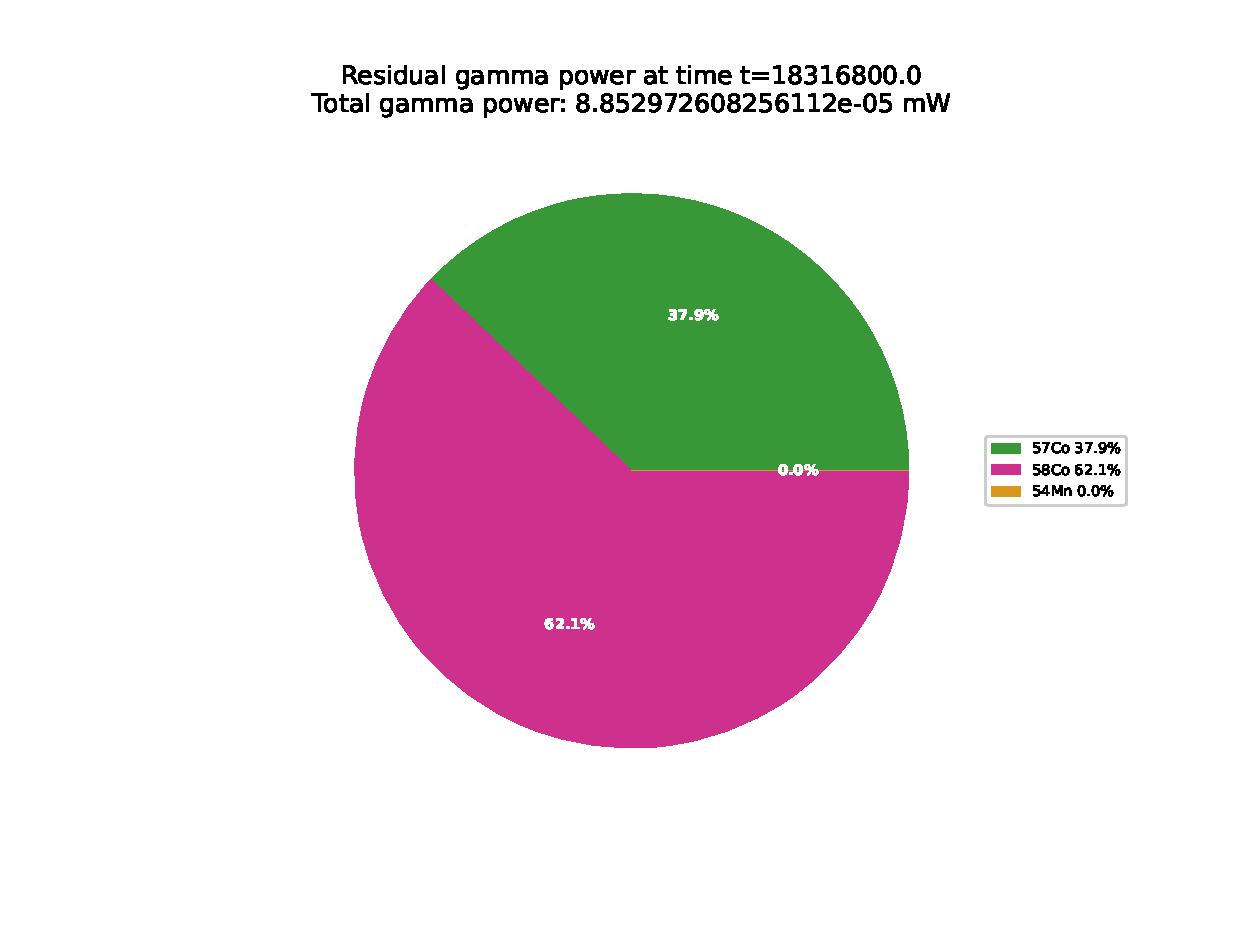
\includegraphics[width=0.7\linewidth]{chapters/activity_code/fe_100dpa/endofbeam/05MeV_0500_18316800.eps}
\caption{}
\label{fig:5mev-proton-100dpa}
\end{figure}


\clearpage
\FloatBarrier
\subsection{10MeV Proton Beam - 60 microamp 100DPA}

The vacancies per ion are at a maximum out of the six settings here with a proton energy of 10MeV.  As a result, the target must be irradiated for just 134 days to reach 100DPA.

\begin{figure}[!htb]
\centering
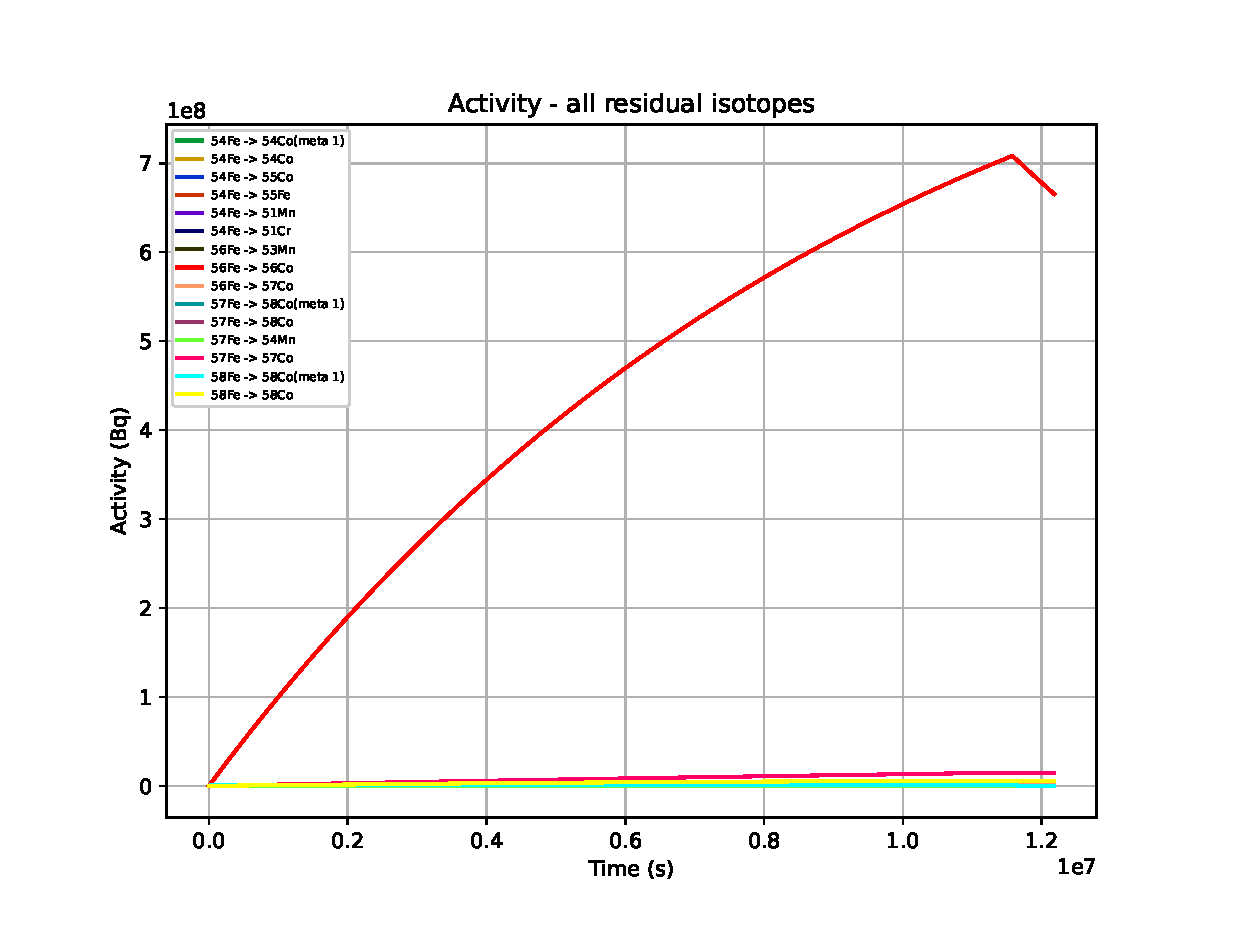
\includegraphics[width=0.7\linewidth]{chapters/activity_code/fe_100dpa/by_isotope/10MeV_all_radioactive_isotopes.eps}
\caption{}
\label{fig:5mev-proton-100dpa-activity}
\end{figure}

\begin{figure}[!htb]
\centering
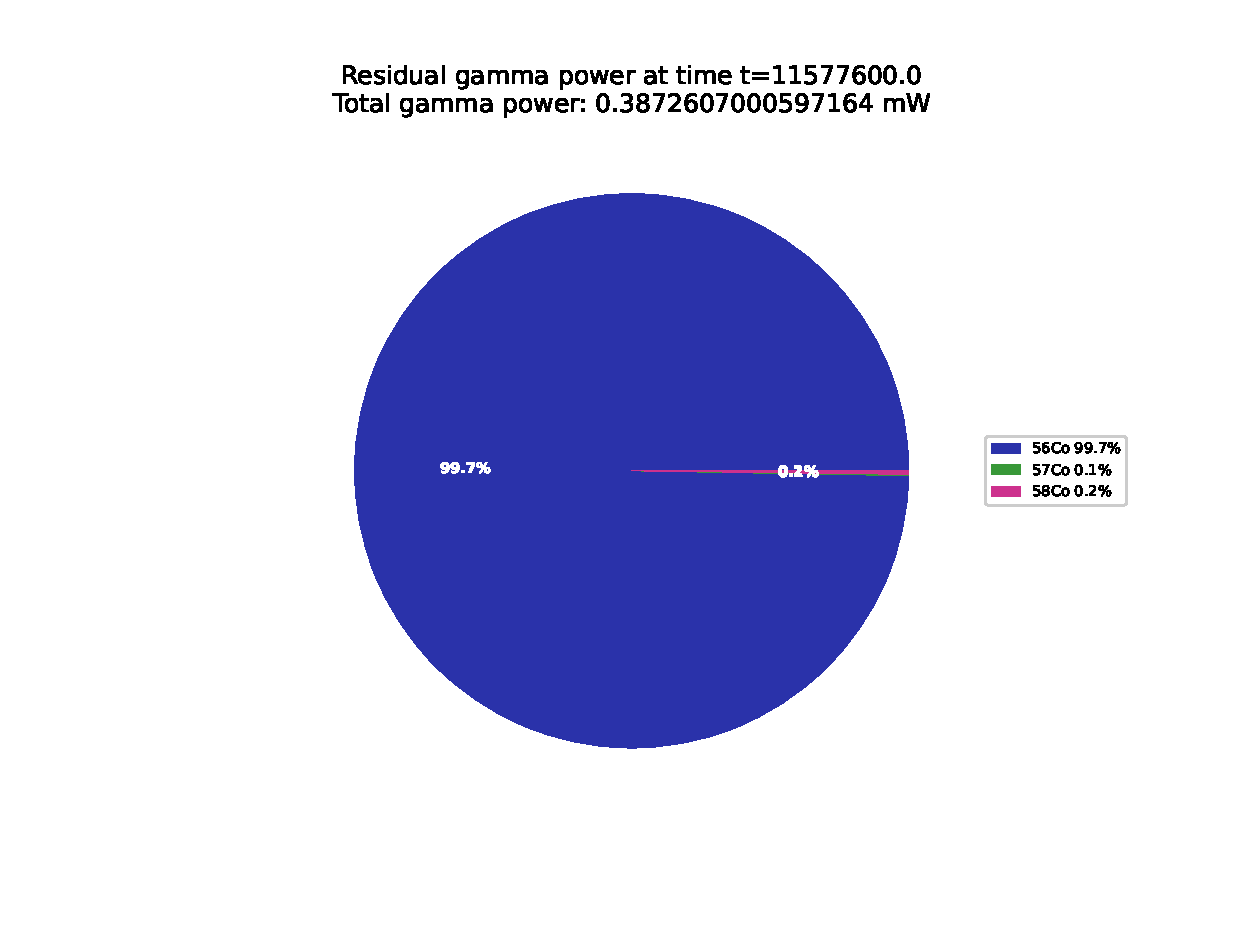
\includegraphics[width=0.7\linewidth]{chapters/activity_code/fe_100dpa/endofbeam/10MeV_0400_11577600.eps}
\caption{}
\label{fig:5mev-proton-100dpa}
\end{figure}

\begin{figure}[!htb]
\centering
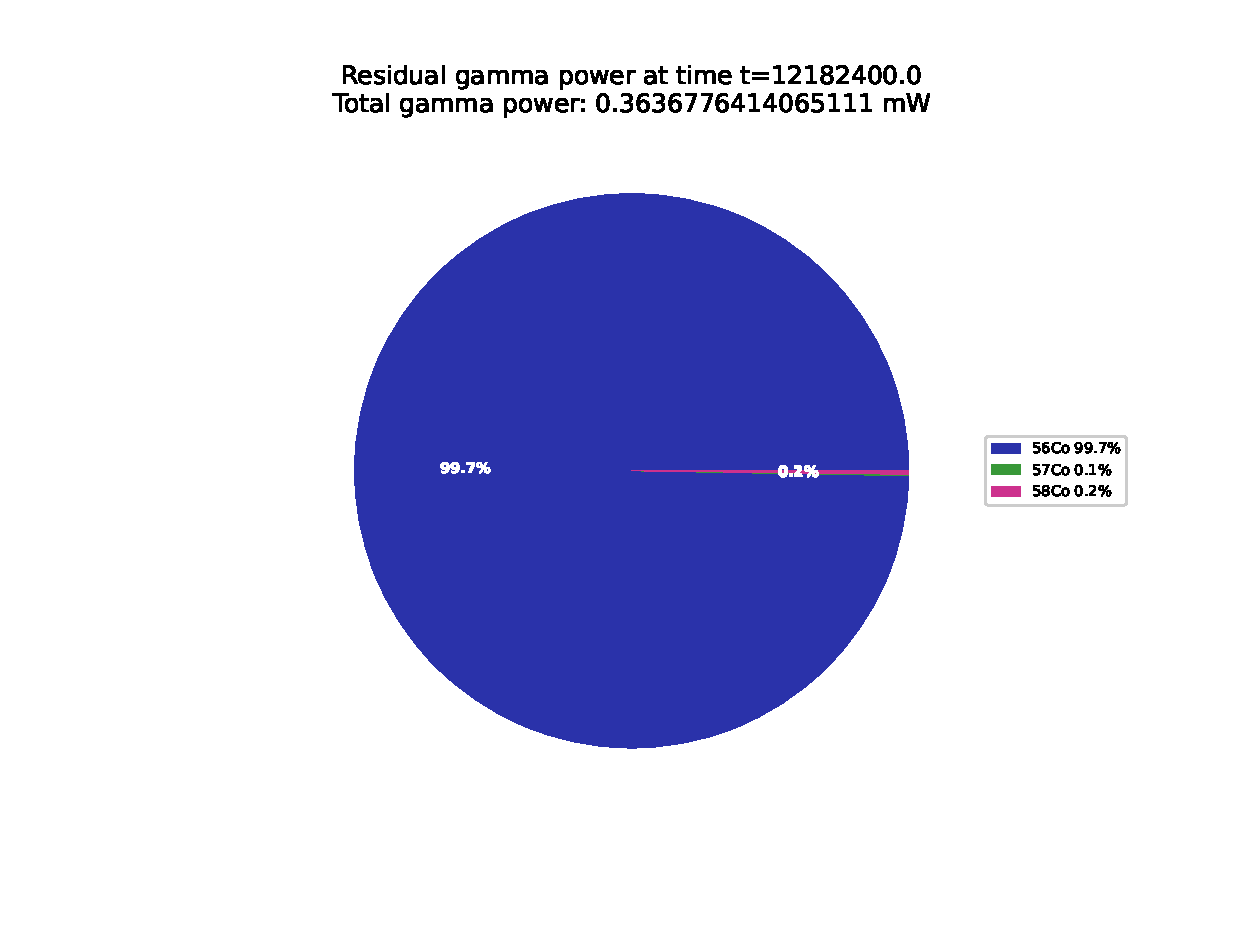
\includegraphics[width=0.7\linewidth]{chapters/activity_code/fe_100dpa/endofbeam/10MeV_0500_12182400.eps}
\caption{}
\label{fig:5mev-proton-100dpa}
\end{figure}



\clearpage
\FloatBarrier
\subsection{15MeV Proton Beam - 60 microamp 100DPA}

\begin{figure}[!htb]
\centering
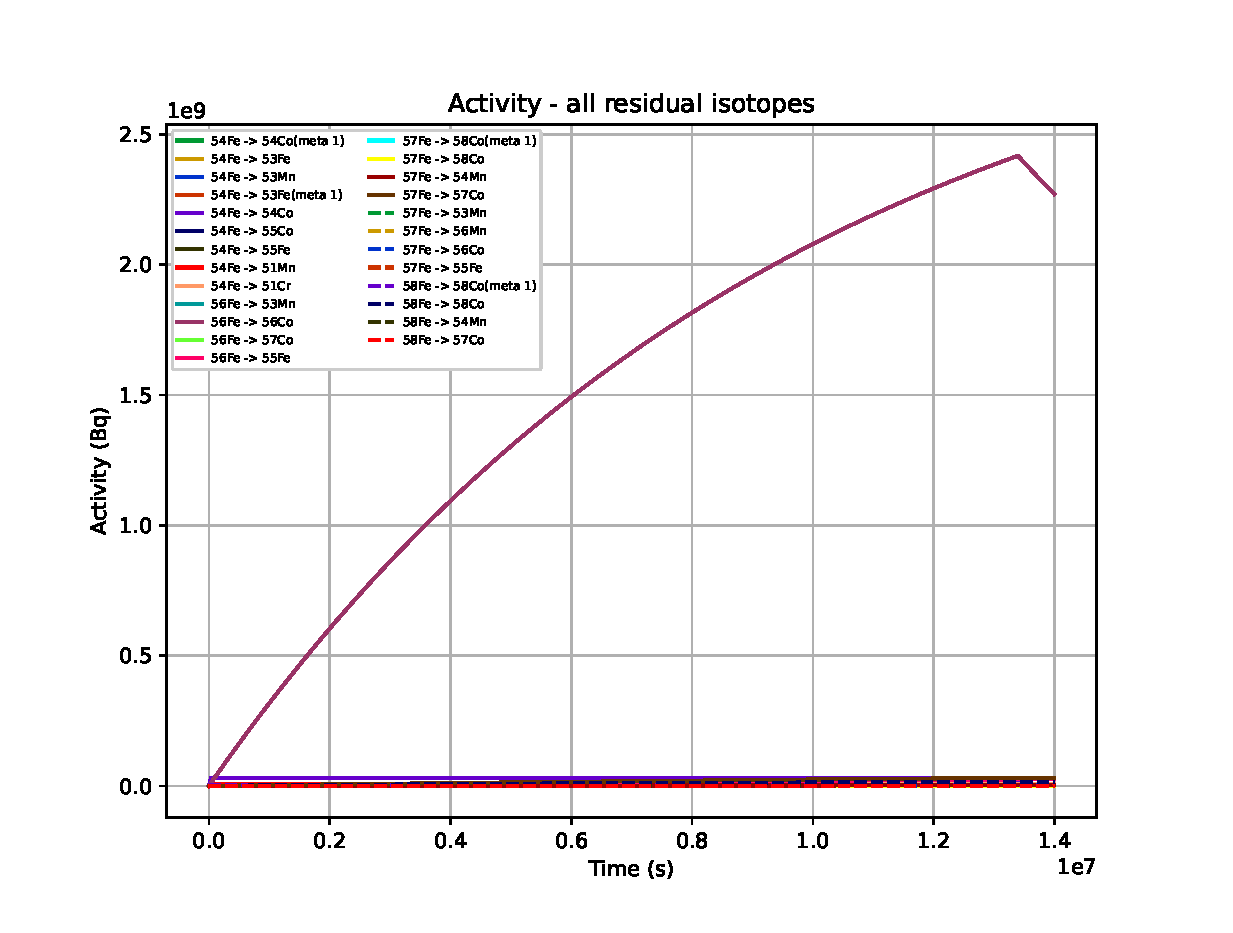
\includegraphics[width=0.7\linewidth]{chapters/activity_code/fe_100dpa/by_isotope/15MeV_all_radioactive_isotopes.eps}
\caption{}
\label{fig:5mev-proton-100dpa-activity}
\end{figure}

\begin{figure}[!htb]
\centering
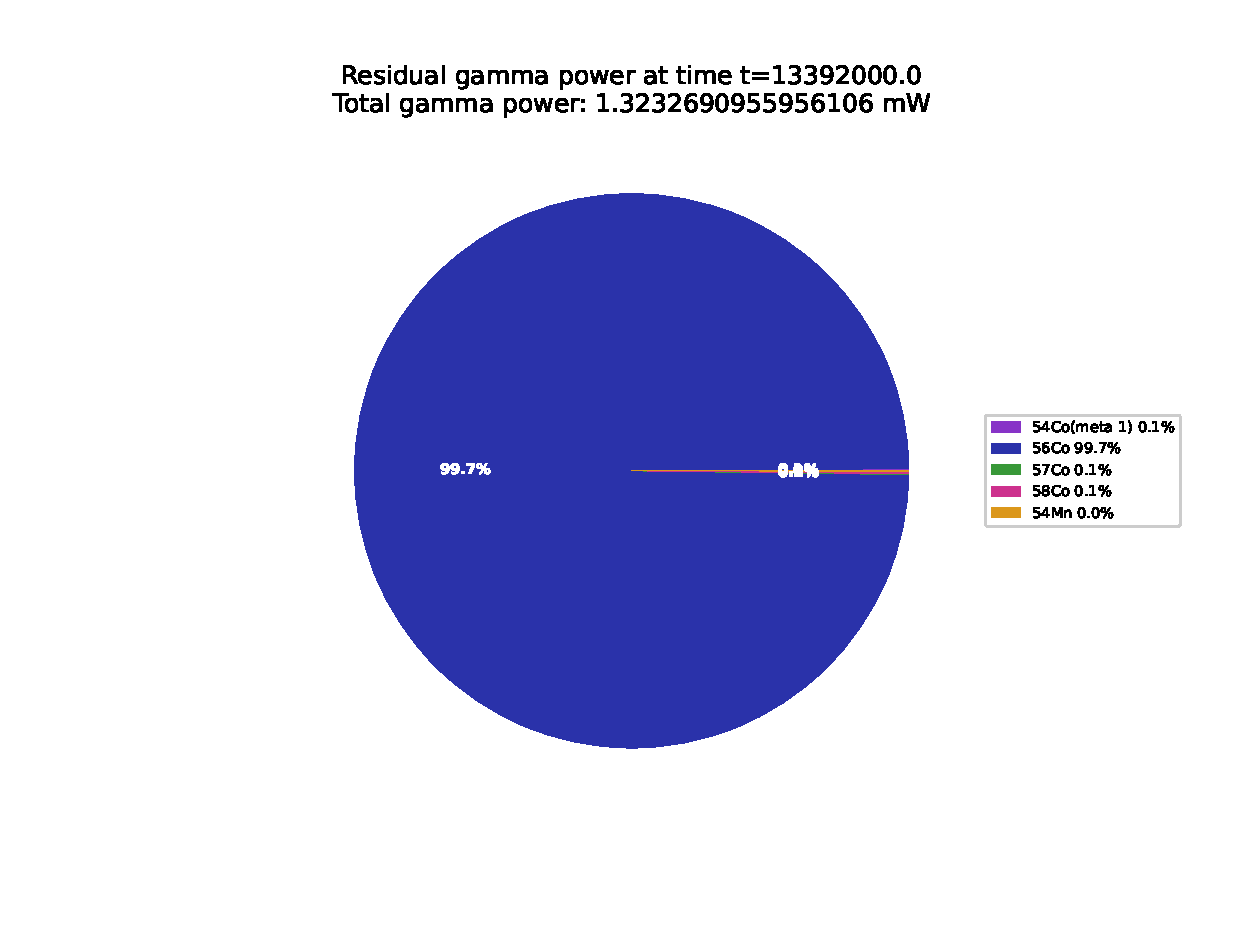
\includegraphics[width=0.7\linewidth]{chapters/activity_code/fe_100dpa/endofbeam/15MeV_0400_13392000.eps}
\caption{}
\label{fig:5mev-proton-100dpa}
\end{figure}

\begin{figure}[!htb]
\centering
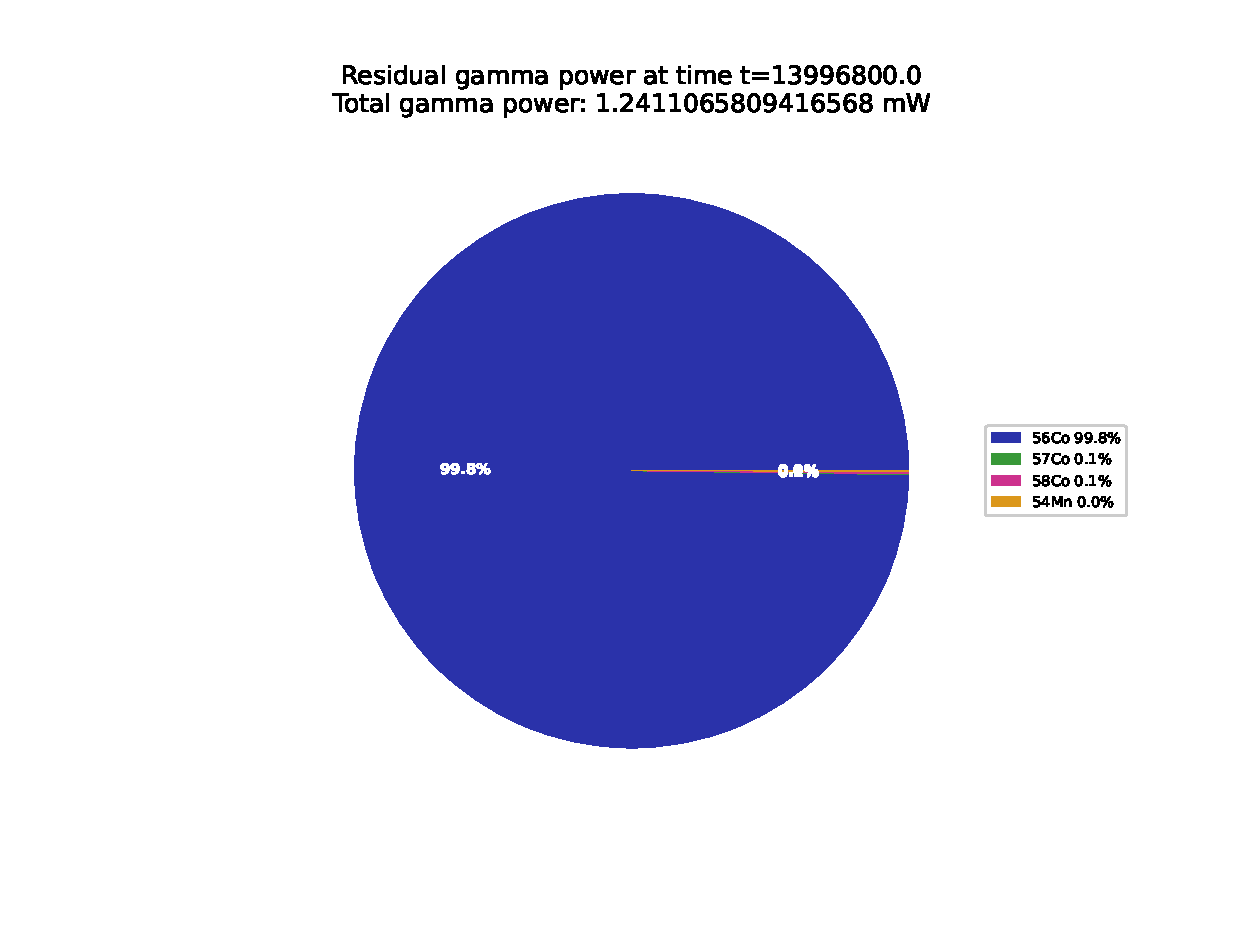
\includegraphics[width=0.7\linewidth]{chapters/activity_code/fe_100dpa/endofbeam/15MeV_0500_13996800.eps}
\caption{}
\label{fig:5mev-proton-100dpa}
\end{figure}



\clearpage
\FloatBarrier
\subsection{20MeV Proton Beam - 60 microamp 100DPA}

\begin{figure}[!htb]
\centering
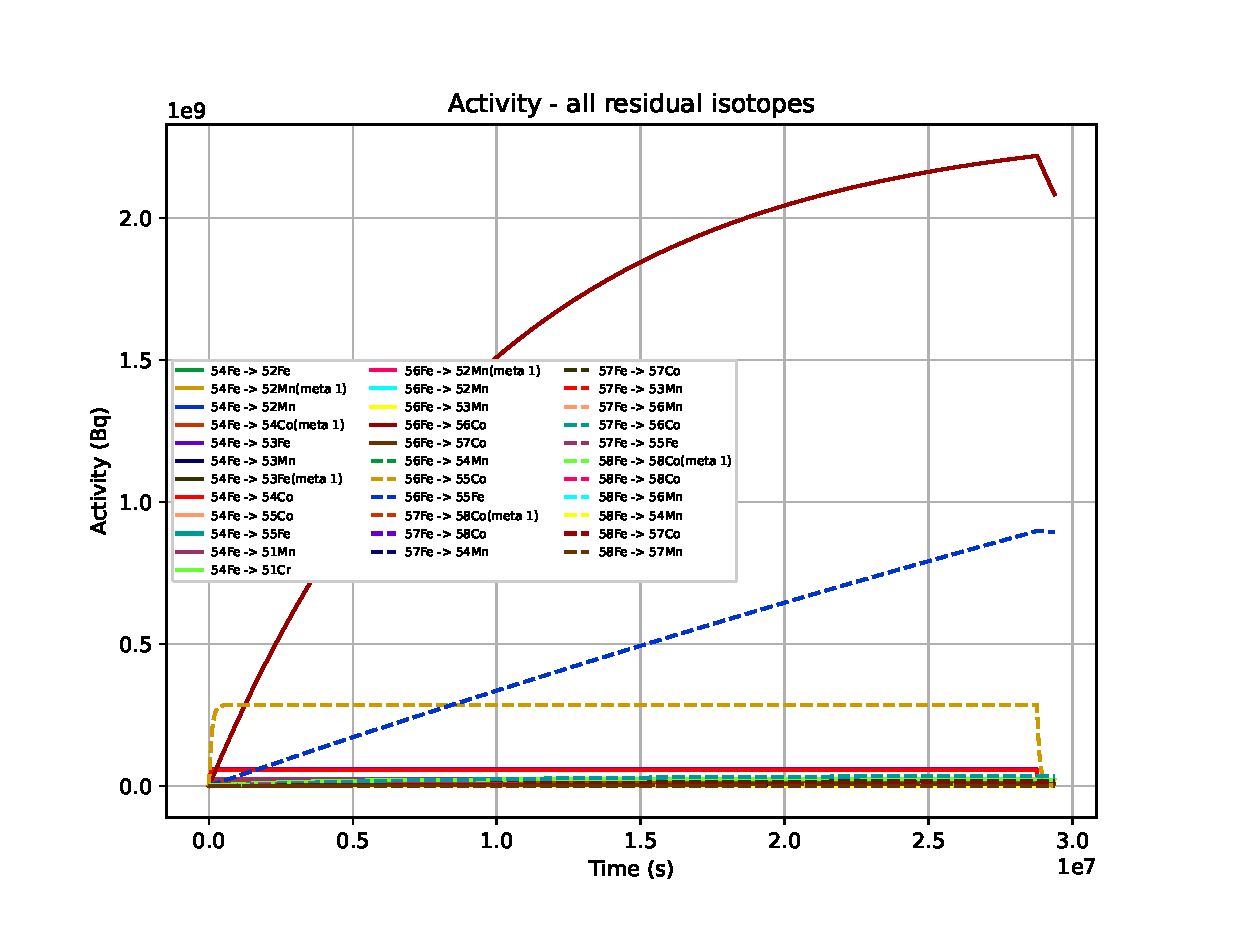
\includegraphics[width=0.7\linewidth]{chapters/activity_code/fe_100dpa/by_isotope/20MeV_all_radioactive_isotopes.eps}
\caption{}
\label{fig:5mev-proton-100dpa-activity}
\end{figure}

\begin{figure}[!htb]
\centering
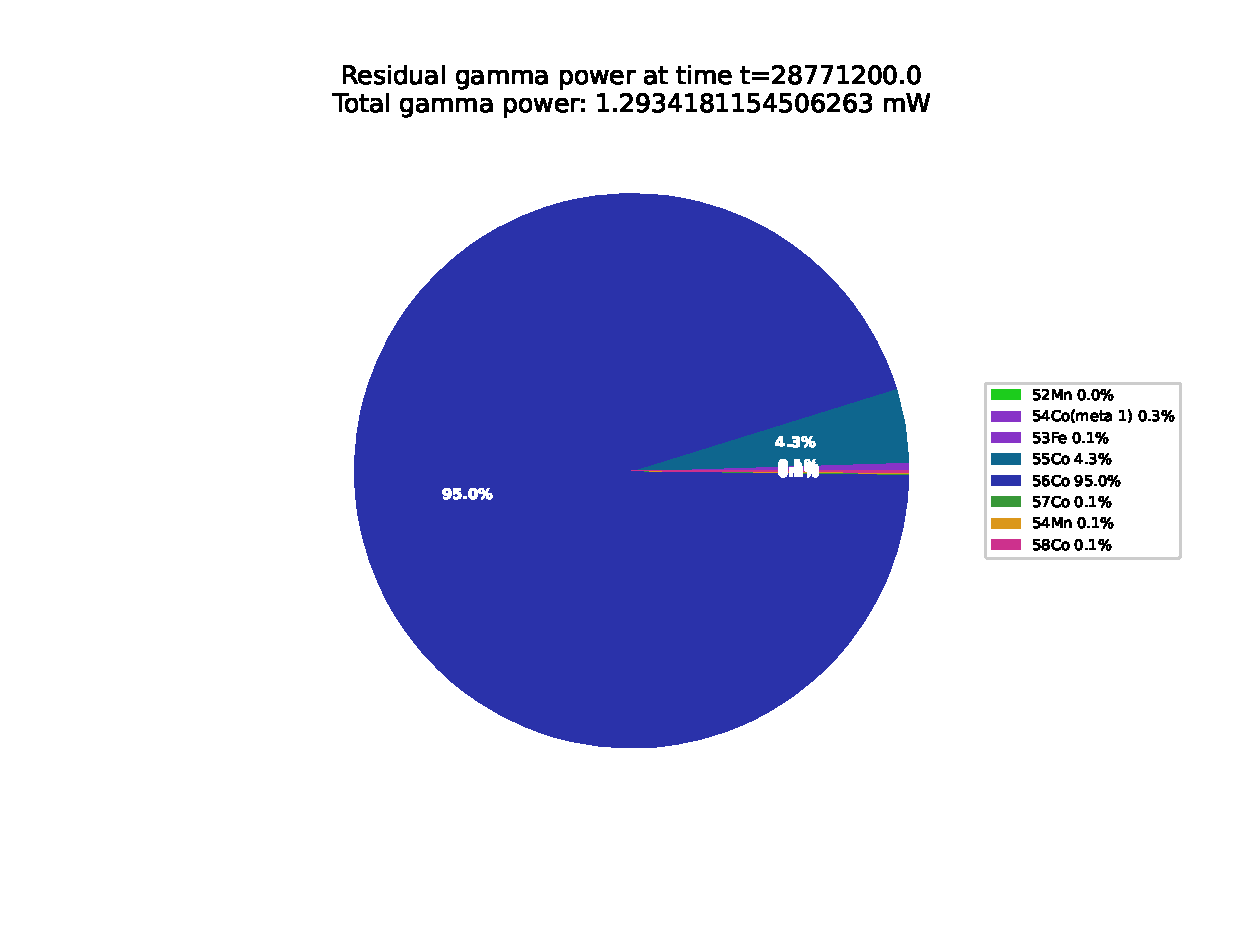
\includegraphics[width=0.7\linewidth]{chapters/activity_code/fe_100dpa/endofbeam/20MeV_0400_28771200.eps}
\caption{}
\label{fig:5mev-proton-100dpa}
\end{figure}

\begin{figure}[!htb]
\centering
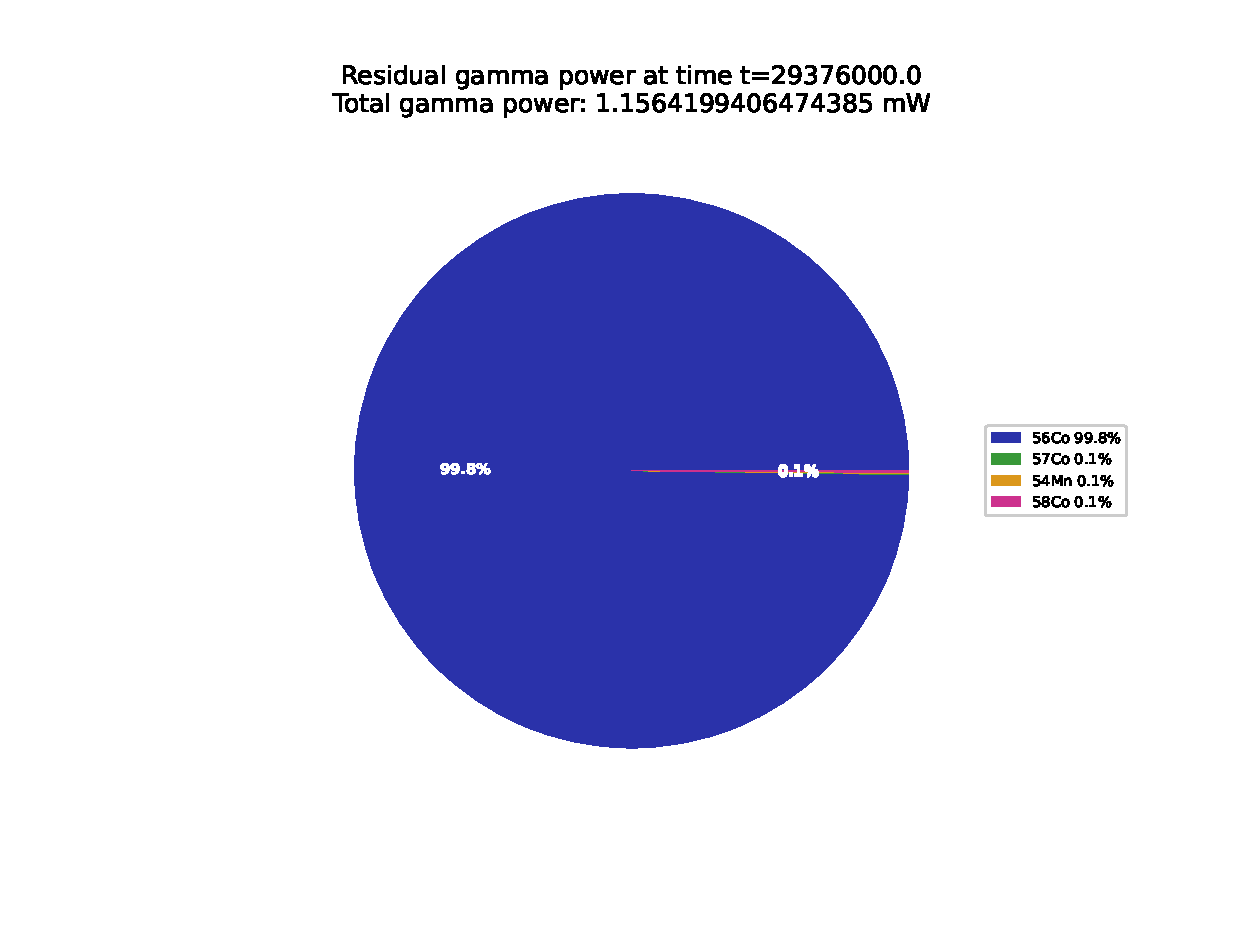
\includegraphics[width=0.7\linewidth]{chapters/activity_code/fe_100dpa/endofbeam/20MeV_0500_29376000.eps}
\caption{}
\label{fig:5mev-proton-100dpa}
\end{figure}



\clearpage
\FloatBarrier
\subsection{25MeV Proton Beam - 60 microamp 100DPA}

\begin{figure}[!htb]
\centering
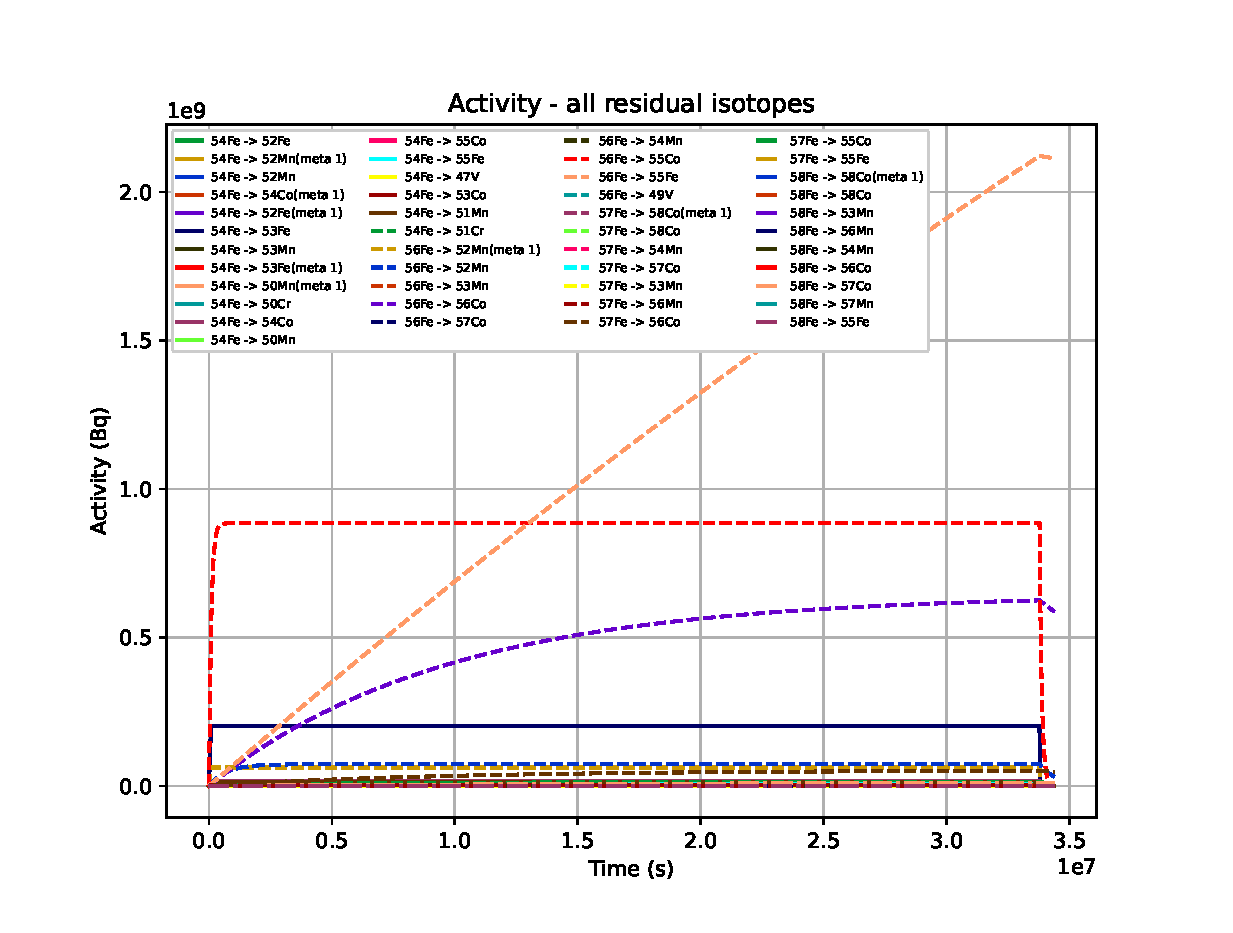
\includegraphics[width=0.7\linewidth]{chapters/activity_code/fe_100dpa/by_isotope/25MeV_all_radioactive_isotopes.eps}
\caption{}
\label{fig:5mev-proton-100dpa-activity}
\end{figure}

\begin{figure}[!htb]
\centering
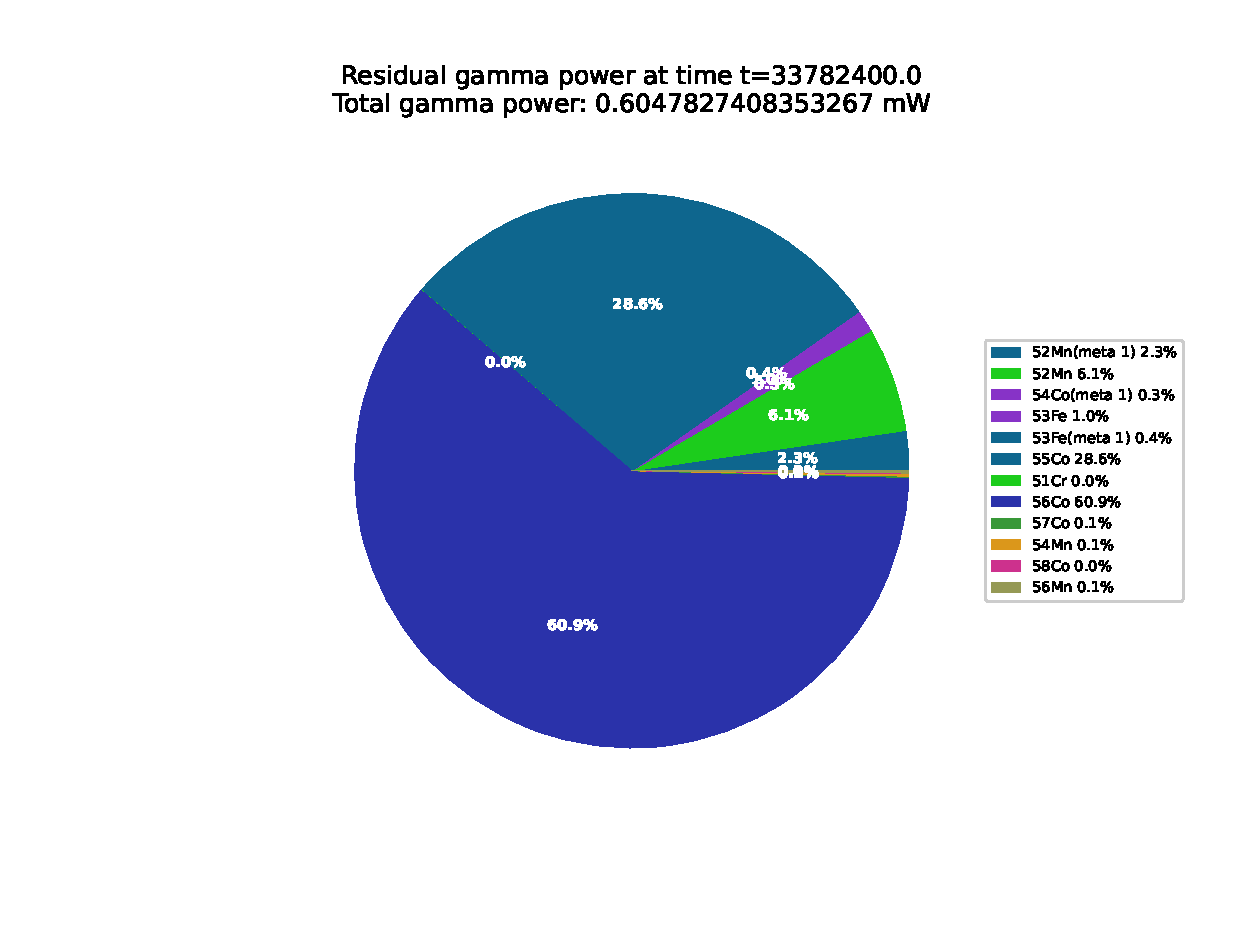
\includegraphics[width=0.7\linewidth]{chapters/activity_code/fe_100dpa/endofbeam/25MeV_0400_33782400.eps}
\caption{}
\label{fig:5mev-proton-100dpa}
\end{figure}

\begin{figure}[!htb]
\centering
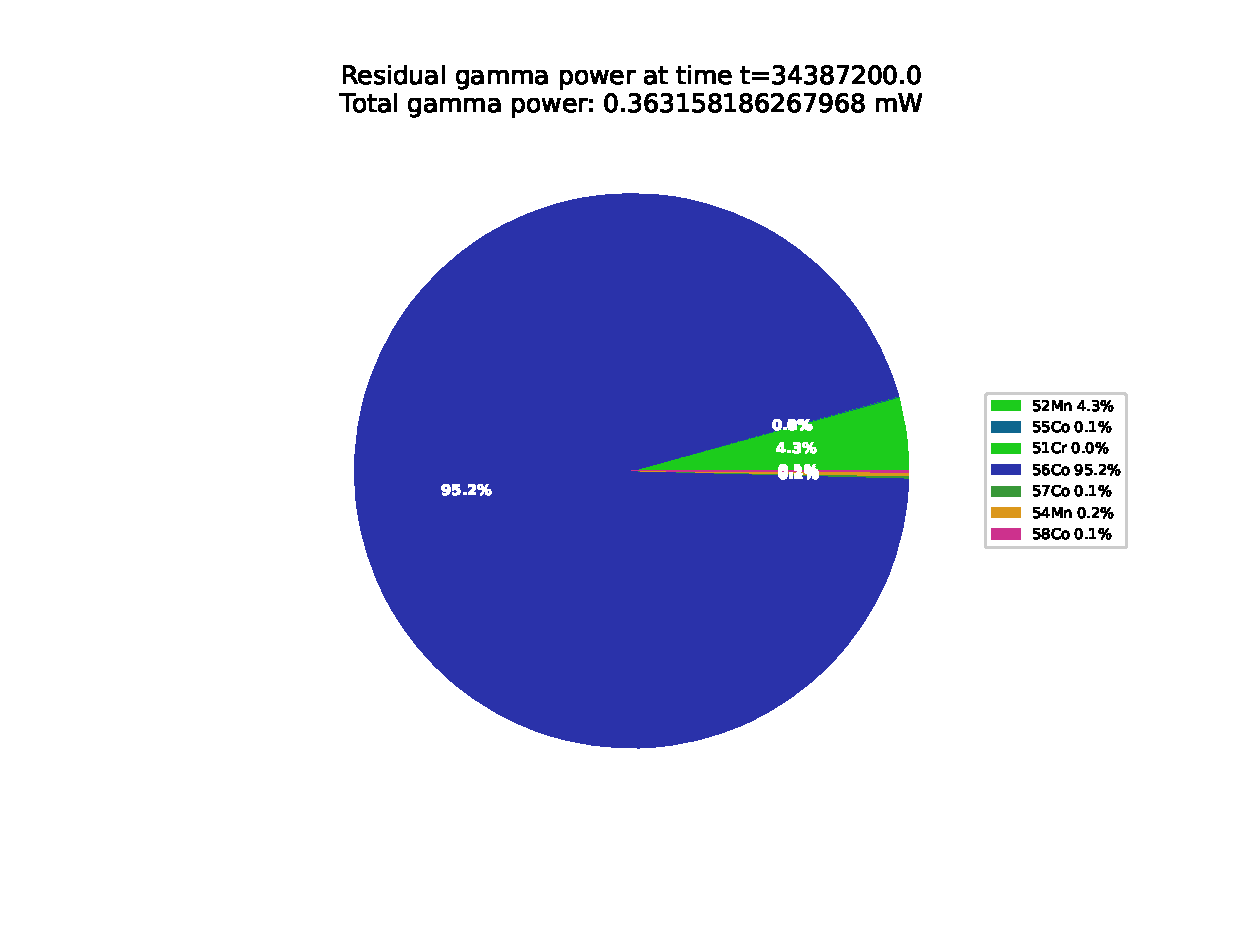
\includegraphics[width=0.7\linewidth]{chapters/activity_code/fe_100dpa/endofbeam/25MeV_0500_34387200.eps}
\caption{}
\label{fig:5mev-proton-100dpa}
\end{figure}



\clearpage
\FloatBarrier
\subsection{30MeV Proton Beam - 60 microamp 100DPA}

\begin{figure}[!htb]
\centering
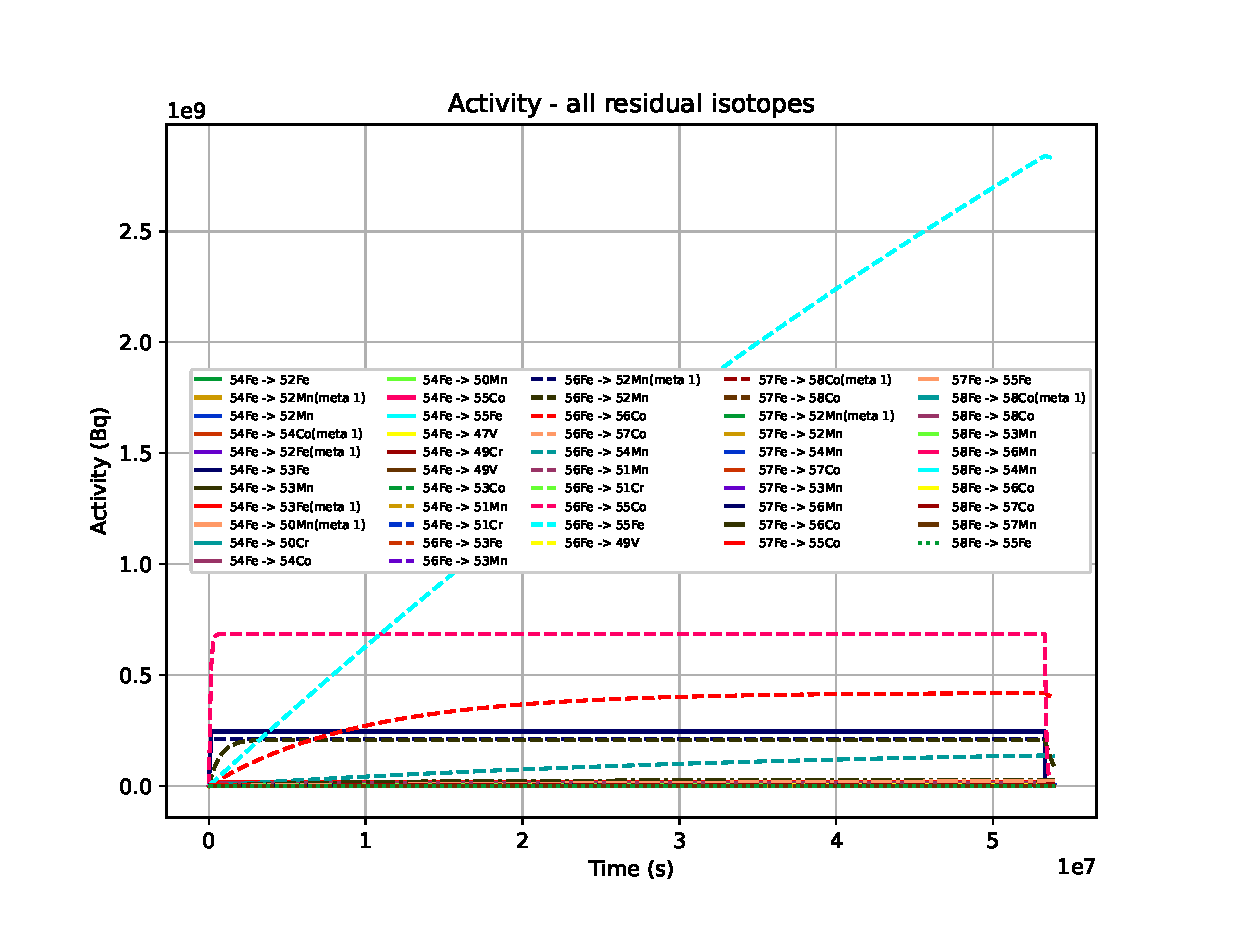
\includegraphics[width=0.7\linewidth]{chapters/activity_code/fe_100dpa/by_isotope/30MeV_all_radioactive_isotopes.eps}
\caption{}
\label{fig:5mev-proton-100dpa-activity}
\end{figure}

\begin{figure}[!htb]
\centering
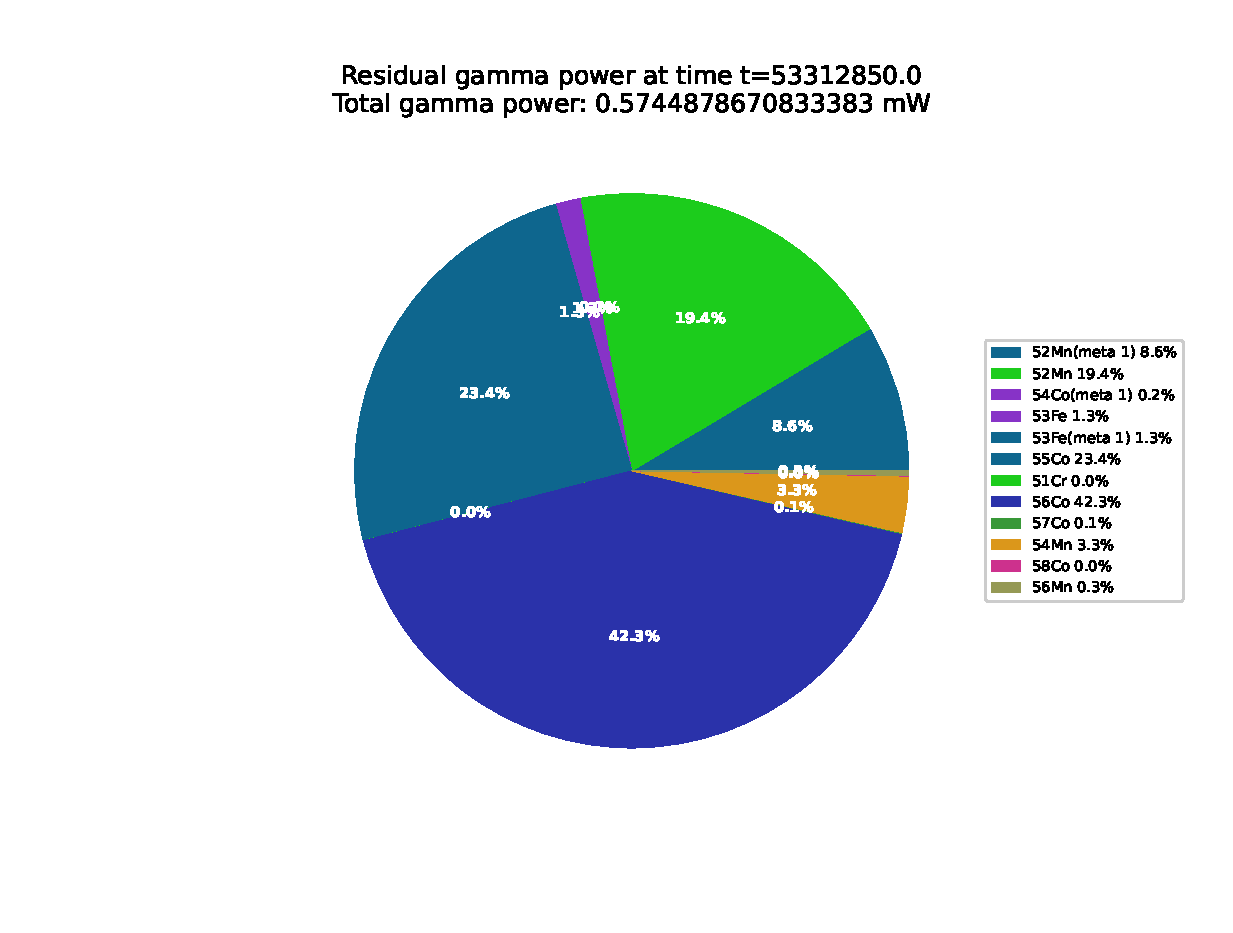
\includegraphics[width=0.7\linewidth]{chapters/activity_code/fe_100dpa/endofbeam/30MeV_0400_53312850.eps}
\caption{}
\label{fig:5mev-proton-100dpa}
\end{figure}

\begin{figure}[!htb]
\centering
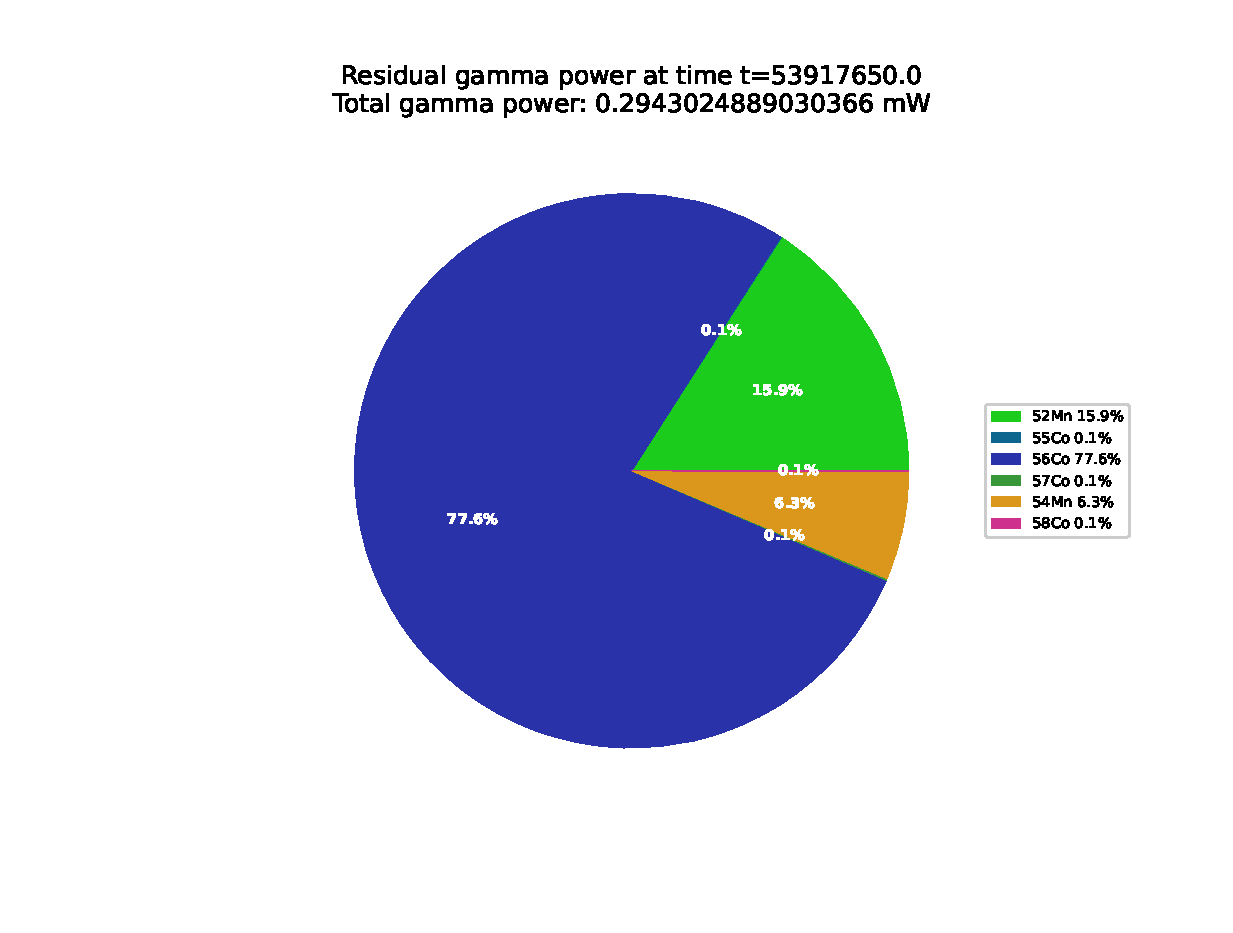
\includegraphics[width=0.7\linewidth]{chapters/activity_code/fe_100dpa/endofbeam/30MeV_0500_53917650.eps}
\caption{}
\label{fig:5mev-proton-100dpa}
\end{figure}



